% ============================================================
%  Training Stability, Not Domain Difference,
%  Determines Linear Mode Connectivity
%  LaTeX source — Draft v12 — 2026-07-14
%  Compile: xelatex paper.tex && xelatex paper.tex
% ============================================================
\documentclass[11pt,a4paper]{article}

% --- Layout ---
\usepackage[margin=2.5cm]{geometry}
\usepackage{setspace}
\onehalfspacing

% --- Typography ---
\usepackage{fontspec}
\IfFontExistsTF{Times New Roman}{%
  \setmainfont{Times New Roman}
}{%
  \setmainfont{Latin Modern Roman}
}
\usepackage{microtype}

% --- Math ---
\usepackage{amsmath,amssymb,amsfonts}
\usepackage{bm}
\usepackage{mathtools}
\DeclareMathOperator*{\argmax}{arg\,max}

% --- Figures ---
\usepackage{graphicx}
\usepackage[font=small,labelfont=bf,skip=4pt]{caption}

% --- Tables ---
\usepackage{booktabs}
\usepackage{siunitx}
\sisetup{detect-all,separate-uncertainty=true}

% --- Colors ---
\usepackage[dvipsnames]{xcolor}
\definecolor{codeblue}{HTML}{2196F3}
\definecolor{medred}{HTML}{F44336}
\definecolor{generalgreen}{HTML}{4CAF50}
\definecolor{mathorange}{HTML}{FF9800}
\definecolor{noisegray}{HTML}{9E9E9E}
\definecolor{purple}{HTML}{9C27B0}

% --- Hyperlinks ---
\usepackage[colorlinks=true,linkcolor=black,citecolor=black,urlcolor=blue]{hyperref}

% --- Headers ---
\usepackage{fancyhdr}
\pagestyle{fancy}
\fancyhf{}
\fancyhead[L]{\small\textit{Training Stability and Linear Mode Connectivity}}
\fancyhead[R]{\small\textit{Draft v12 — \today}}
\fancyfoot[C]{\thepage}
\renewcommand{\headrulewidth}{0.4pt}

% --- Title ---
\title{\textbf{Training Stability, Not Domain Difference,\\[4pt]
               Determines Linear Mode Connectivity}\\[8pt]
       \large Draft v12 — \today}

\author{}
\date{}

\begin{document}
\maketitle
\thispagestyle{fancy}

% ============================================================
% ABSTRACT
% ============================================================
\begin{center}
\rule{0.95\textwidth}{0.5pt}\\[4pt]
\begin{minipage}{0.92\textwidth}
\small
When a pretrained language model is fine-tuned on different domains, how far do the resulting models move in weight space? Do they remain in the same linearly-connected loss basin? We measure this on Pythia-1.4B fine-tuned on code and medical reasoning tasks. At standard training intensity, the models diverge by 1.4--1.5\% in weight space and the LMC barrier is 0.05 — well within the linearly-connected regime. At higher divergence (8.0--8.5\% weight displacement, 11.6\% cross-model), the barrier rises to $0.12 \pm 0.03$ (code) and $0.23 \pm 0.10$ (medical) — a 2--5$\times$ increase. However, even at this divergence level the barrier remains modest, suggesting that domain specialization alone does not easily break linear connectivity. Within-domain baselines reveal a striking asymmetry: code models exhibit near-identical barriers within and across domains ($0.048$ vs.\ $0.053$), while medical models show 3$\times$ larger within-domain than cross-domain barriers ($0.147$ vs.\ $0.051$). This indicates that training stability, not domain difference, is the dominant source of LMC barrier height — and that stability varies dramatically across domains. Noise-floor calibration places these results in context: identical copies yield barrier $\approx 0.000$, and pretrained-to-random-init interpolation provides a reference point of $0.150 \pm 0.019$ (3-seed calibration). Per-block divergence patterns are nearly identical across domains ($r = 0.995$). A training trajectory analysis reveals that the barrier follows an inverted-U shape for code (peaking mid-training then declining) but grows monotonically for medical — confirming domain-specific stability at the within-run level. Gaussian perturbation experiments show that unstructured noise produces negligible barriers even at 8\% weight displacement, while structured training-induced changes create barriers 9$\times$ larger at equivalent magnitude. Layer-selective interpolation demonstrates that the barrier is almost entirely concentrated in early transformer layers (0--7), with deep layers (16--23) showing near-zero interpolation penalty — a directly actionable finding for model merging practice.
\end{minipage}\\[4pt]
\rule{0.95\textwidth}{0.5pt}
\end{center}

% ============================================================
% 1. INTRODUCTION
% ============================================================
\section{Introduction}

Fine-tuning pretrained language models on domain-specific data produces specialized capabilities. But how far do these fine-tuned models actually move from their starting point? When two models are fine-tuned on different domains, does the linear path between their weights cross a loss barrier — or do they remain in the same basin?

Linear Mode Connectivity~\cite{frankle2020lmc} established that neural networks fine-tuned from the same initialization often lie in the same linearly-connected loss basin. Subsequent work~\cite{wortsman2022soups,yadav2023ties} showed that weight interpolation between related models can even improve performance. But the quantitative relationship between \emph{how much} models diverge in weight space and \emph{whether} they remain connected remains underexplored.

We measure this relationship directly. Using Pythia-1.4B as a base model, we train two variants on code reasoning and medical reasoning respectively. We vary the degree of weight-space movement, measure per-block divergence from the pretrained checkpoint, and compute LMC barriers via 11-point linear interpolation between the domain-specialized models.

Our contributions are:
\begin{enumerate}
    \item The first systematic measurement of how quantitative weight displacement maps onto LMC barrier height in fine-tuned language models, spanning four divergence levels (1.4\%--8\%), four domains (code, general, math, medical), and 24+ trained models.
    \item The discovery that training stability — not domain difference — is the dominant source of LMC barrier height, with medical-domain training producing 3$\times$ larger within-domain than cross-domain barriers. Seed-pair analysis ($n = 5$, 10 pairs) reveals a 15$\times$ barrier range depending on partner compatibility.
    \item Mechanistic characterization via training trajectory analysis (inverted-U for code vs.\ monotonic growth for medical), Gaussian perturbation calibration (structured displacement creates 9$\times$ larger barriers than unstructured noise at equivalent magnitude), and layer-selective interpolation (75\% of the barrier concentrated in the first 8 transformer layers).
\end{enumerate}

% ============================================================
% 2. RELATED WORK
% ============================================================
\section{Related Work}

\subsection{Linear Mode Connectivity}

Draxler et al.~\cite{draxler2018barriers} first demonstrated empirically that neural network minima are connected by near-zero-barrier paths. Garipov et al.~\cite{garipov2018loss} introduced Fast Geometric Ensembling via B\'{e}zier curves. Frankle et al.~\cite{frankle2020lmc} formalized the linear interpolation barrier definition we adopt. Li et al.~\cite{li2018visualizing} provided the standard visualization framework for loss landscapes. Entezari et al.~\cite{entezari2022permutation} proved that permutation symmetry accounts for most apparent LMC failures — fine-tuned models from the same initialization are almost certainly connected after permutation alignment. Ainsworth et al.~\cite{ainsworth2023git} operationalized this with Git Re-Basin matching algorithms. Mirzadeh et al.~\cite{mirzadeh2021lmc} studied LMC in continual learning settings. Lubana et al.~\cite{lubana2023mechanistic} provided mechanistic explanations for when mode connectivity holds. Our work differs by measuring how \emph{quantitative weight displacement} maps onto LMC barrier height, rather than testing connectivity as a binary property.

\subsection{Model Merging}

Linear weight interpolation has proven practically useful. Izmailov et al.~\cite{izmailov2018averaging} showed weight averaging finds wider optima (SWA). Wortsman et al.~\cite{wortsman2022soups} averaged fine-tuned variants into ``Model Soups'' that improve robustness at zero inference cost. Wortsman et al.~\cite{wortsman2022wise} demonstrated (WiSE-FT) that interpolating zero-shot and fine-tuned weights improves distribution shift robustness. Yadav et al.~\cite{yadav2023ties} introduced TIES-Merging, resolving parameter interference through trim-elect-sign operations. Task arithmetic~\cite{ilharco2023editing} showed weight-space vector addition composes task capabilities. Matena \& Raffel~\cite{matena2022merging} proposed Fisher-weighted averaging grounded in Laplace posterior approximation. Jin et al.~\cite{jin2023dataless} demonstrated dataless knowledge fusion via weight merging, and Stoica et al.~\cite{stoica2024zipit} merged models from different tasks without training (ZipIt!). These methods demonstrate that weight-space operations \emph{work}, but do not characterize \emph{when they fail}. Our barrier measurements provide a quantitative framework connecting weight divergence magnitude to expected interpolation quality — a predictor that could guide practitioners in deciding when to merge.

\subsection{Fine-Tuning Analysis}

Neyshabur et al.~\cite{neyshabur2020transfer} investigated what is transferred during fine-tuning, finding that feature reuse rather than task-specific adaptation dominates. Gururangan et al.~\cite{gururangan2020dapt} established domain-adaptive pretraining (DAPT) as the standard paradigm, but focused on downstream accuracy, not weight-space properties. Kirkpatrick et al.~\cite{kirkpatrick2017ewc} introduced Elastic Weight Consolidation (EWC) with a Fisher-information framework for measuring parameter importance. Aljundi et al.~\cite{aljundi2018mas} proposed Memory Aware Synapses (MAS), which estimates parameter importance from output sensitivity without requiring labels — a precursor to our per-block divergence analysis. Biderman et al.~\cite{biderman2023pythia} released Pythia checkpoints at multiple training steps with documented training dynamics, enabling the systematic weight-space analysis we leverage. Fort et al.~\cite{fort2019stiffness} introduced ``stiffness'' as a measure of parameter sensitivity. Our work bridges these literatures by measuring how far domain fine-tuning moves models in weight space, characterizing per-block divergence patterns, and connecting displacement magnitude to loss landscape connectivity.

% ============================================================
% 3. METHOD
% ============================================================
\section{Method}

\subsection{Problem Formulation}

Let $\theta_0 \in \mathbb{R}^d$ denote the parameters of a pretrained language model with $d$ total parameters. We fine-tune this model on domain-specific data, yielding a specialized model $\theta \in \mathbb{R}^d$. The weight displacement is defined as the relative $\ell_2$ distance from the pretrained initialization:

\begin{equation}\label{eq:dw}
\Delta W(\theta, \theta_0) = \frac{\|\theta - \theta_0\|_2}{\|\theta_0\|_2} \times 100\%
\end{equation}

For models fine-tuned on domains $A$ and $B$, yielding $\theta_A$ and $\theta_B$, we define the cross-model divergence:
\begin{equation}
\Delta W_{\text{cross}}(\theta_A, \theta_B) = \frac{\|\theta_A - \theta_B\|_2}{\|\theta_0\|_2} \times 100\%
\end{equation}

\subsection{Linear Mode Connectivity Barrier}

For two models $\theta_A, \theta_B \in \mathbb{R}^d$, we construct an interpolated model at mixing ratio $\alpha \in [0, 1]$:

\begin{equation}\label{eq:interp}
\theta(\alpha) = (1 - \alpha) \cdot \theta_A + \alpha \cdot \theta_B
\end{equation}

We evaluate the binary cross-entropy loss $\mathcal{L}(\theta(\alpha))$ on a held-out test set of 2,000 samples per domain. The LMC barrier follows Frankle et al.~\cite{frankle2020lmc}:

\begin{equation}\label{eq:barrier}
\boxed{\mathcal{B}(\theta_A, \theta_B) = \max_{\alpha \in [0,1]} \mathcal{L}\big(\theta(\alpha)\big) - \frac{\mathcal{L}(\theta_A) + \mathcal{L}(\theta_B)}{2}}
\end{equation}

The barrier measures the maximum excess loss along the linear interpolation path relative to the endpoint average. A barrier of zero indicates perfect linear connectivity; larger barriers indicate degradation when interpolating. In practice, we sample $\alpha \in \{0.0, 0.1, \dots, 1.0\}$ (11 points).

\subsection{Per-Block Divergence}

For a transformer with $L$ layers, let $\theta^{(\ell)} \subset \theta$ denote the parameters of layer $\ell$. The per-block weight divergence is:

\begin{equation}\label{eq:perblock}
\Delta W^{(\ell)} = \frac{\|\theta^{(\ell)} - \theta_0^{(\ell)}\|_2}{\|\theta_0^{(\ell)}\|_2} \times 100\%, \quad \ell = 0, 1, \dots, L-1
\end{equation}

The Pearson correlation $r$ between per-block divergence vectors from two domains quantifies the similarity of their layer-wise change patterns:
\begin{equation}
r = \frac{\sum_{\ell} (\Delta W_A^{(\ell)} - \overline{\Delta W}_A)(\Delta W_B^{(\ell)} - \overline{\Delta W}_B)}{\sqrt{\sum_{\ell}(\Delta W_A^{(\ell)} - \overline{\Delta W}_A)^2} \sqrt{\sum_{\ell}(\Delta W_B^{(\ell)} - \overline{\Delta W}_B)^2}}
\end{equation}

\subsection{Gaussian Perturbation Baseline}

To disentangle the effects of weight displacement \emph{magnitude} from \emph{directional structure}, we construct a perturbed model via isotropic Gaussian noise:

\begin{equation}\label{eq:gaussian}
\theta_{\text{noise}} = \theta_0 + \sigma \cdot \bm{\epsilon}, \quad \bm{\epsilon} \sim \mathcal{N}(0, \mathbf{I}_d)
\end{equation}

where $\sigma$ is chosen such that $\Delta W(\theta_{\text{noise}}, \theta_0)$ matches a target displacement level. The barrier $\mathcal{B}(\theta_0, \theta_{\text{noise}})$ measures the effect of \emph{unstructured} weight displacement, providing a baseline against which training-induced (structured) displacement can be compared.

\subsection{Layer-Selective Interpolation}

For a subset of layers $\mathcal{S} \subseteq \{0, \dots, L-1\}$, we construct the partially-merged model:

\begin{equation}\label{eq:layersel}
\theta^{(\ell)}_{\mathcal{S}}(\alpha) = \begin{cases}
(1 - \alpha) \theta_A^{(\ell)} + \alpha \theta_B^{(\ell)} & \text{if } \ell \in \mathcal{S} \\[4pt]
\theta_A^{(\ell)} & \text{if } \ell \notin \mathcal{S}
\end{cases}
\end{equation}

The barrier $\mathcal{B}_{\mathcal{S}} = \mathcal{B}(\theta_{\mathcal{S}}(0), \theta_{\mathcal{S}}(1))$ isolates the contribution of layer group $\mathcal{S}$ to the total interpolation penalty.

\subsection{Training Trajectory Analysis}

During a single training run, we save checkpoints $\theta^{(t)}$ at steps $t = 40, 80, \dots, 400$ and measure the barrier against the pretrained base model:

\begin{equation}\label{eq:traj}
\mathcal{B}_{\text{traj}}(t) = \mathcal{B}\big(\theta_0,\; \theta^{(t)}\big)
\end{equation}

This yields a continuous $\Delta W \to \mathcal{B}$ curve from a \emph{single} optimization trajectory, eliminating the convergence confound of cross-run comparisons — all checkpoints share the same optimization path.

\subsection{Statistical Framework}

We compare barrier distributions using Welch's $t$-test (unequal variances not assumed) and report Cohen's $d$ as a standardized effect size:

\begin{equation}\label{eq:cohensd}
d = \frac{\bar{x}_1 - \bar{x}_2}{s_p}, \qquad
s_p = \sqrt{\frac{(n_1 - 1)s_1^2 + (n_2 - 1)s_2^2}{n_1 + n_2 - 2}}
\end{equation}

Effect sizes are interpreted following convention: $|d| > 0.8$ (large), $|d| > 0.5$ (medium), $|d| > 0.2$ (small). Bootstrap confidence intervals (100,000 resamples, 95\% CI) are reported for all barrier estimates.

\subsection{Training Configuration}

\begin{table}[h]
\centering
\caption{Training hyperparameters.}
\label{tab:training}
\begin{tabular}{@{}ll@{}}
\toprule
\textbf{Parameter} & \textbf{Value} \\
\midrule
Base model & EleutherAI/pythia-1.4b (1.31B params) \\
Training regime & Full-parameter fine-tuning, 1 epoch \\
Training data & VersaPRM: code (55K train) + medical ($\sim$55K train) \\
Precision & bfloat16 autocast, fp32 classification head \\
Batch size & 128 \\
Sequence length & 256 tokens \\
Optimizer & AdamW ($\beta_1 = 0.9, \beta_2 = 0.999$, weight decay = 0.1) \\
Hardware & NVIDIA DGX Spark GB10 (121GB unified, ARM64 CUDA 13.0) \\
Seeds & 3 per condition (5 for high-divergence medical) \\
\bottomrule
\end{tabular}
\end{table}

Model pairs are created at two divergence levels by varying the optimization step size. We refer to these as the \textbf{standard-divergence} ($\Delta W \approx 1.4\%$) and \textbf{high-divergence} ($\Delta W \approx 8\%$) conditions. The step size values are incidental — what matters is the resulting weight-space distance between models.

% ============================================================
% 4. RESULTS
% ============================================================
\section{Results}

\subsection{Weight Divergence}

\begin{table}[h]
\centering
\caption{Weight displacement from pretrained checkpoint. Cross-model divergence between code and medical variants. Mean $\pm$ 1$\sigma$ over 3 seeds.}
\label{tab:dw}
\begin{tabular}{@{}lccc@{}}
\toprule
\textbf{Condition} & \textbf{Code $\Delta W$} & \textbf{Medical $\Delta W$} & \textbf{Code$\leftrightarrow$Med Cross} \\
\midrule
Standard & $1.4 \pm 0.0\%$ & $1.5 \pm 0.1\%$ & $2.0 \pm 0.1\%$ \\
High     & $8.0 \pm 0.3\%$ & $8.5 \pm 0.2\%$ & $11.6 \pm 0.3\%$ \\
\bottomrule
\end{tabular}
\end{table}

Per-block divergence patterns are nearly identical across domains ($r = 0.995$). Both models change the same transformer blocks; the divergence is primarily in magnitude, not pattern. Divergence concentrates in early layers (layer 0: $\sim$5.6\% at standard divergence) and decreases roughly exponentially with depth (Figure~\ref{fig:fig1}, Panel F).

\subsection{LMC Barriers}

\begin{table}[h]
\centering
\caption{LMC barriers for cross-domain interpolation. Mean $\pm$ 1$\sigma$ over 3 seeds.}
\label{tab:barriers}
\begin{tabular}{@{}lcc@{}}
\toprule
\textbf{Condition} & \textbf{Code barrier} & \textbf{Medical barrier} \\
\midrule
Standard & $0.053 \pm 0.011$ & $0.051 \pm 0.013$ \\
High     & $0.118 \pm 0.031$ & $0.228 \pm 0.102$ \\
\bottomrule
\end{tabular}
\end{table}

Key observations from the barrier measurements:
\begin{enumerate}
    \item At standard divergence ($\Delta W \approx 1.4\%$), LMC holds cleanly: barriers are $\sim$0.05, well within the linearly-connected regime.
    \item At high divergence ($\Delta W \approx 8\%$), barriers increase 2--5$\times$ but remain modest (Figure~\ref{fig:fig1}, Panels A--D).
    \item The barrier grows \emph{less than proportionally} to divergence: 5--6$\times$ more weight displacement yields only 2--5$\times$ more barrier.
    \item At intermediate divergence ($\Delta W \approx 5\%$), we observe seed-dependent catastrophic barrier spikes: three code models with near-identical weight displacement ($\Delta W \approx 4.6\%$) produce barriers of 0.056, 0.096, and 1.043 — a 19$\times$ range. The model with the highest barrier (1.043) has the \emph{best} self-domain performance (loss 0.566 vs.\ 0.584--0.595), indicating that catastrophic interpolation failure can coexist with strong task-specific convergence.
\end{enumerate}

\subsection{Within-Domain LMC Baseline}

To calibrate the cross-domain barriers, we measure LMC between different seeds of the \emph{same} domain (3 pairs each, standard divergence). We extend this analysis to two additional domains (math and general reasoning) to test whether the stability pattern generalizes:

\begin{table}[h]
\centering
\caption{Within-domain LMC barriers across four domains.}
\label{tab:within}
\begin{tabular}{@{}lcc@{}}
\toprule
\textbf{Domain} & \textbf{Barrier} & \textbf{Interpretation} \\
\midrule
Code    & $0.048 \pm 0.000$ & Highly stable — near-zero seed variance \\
General & $0.071 \pm 0.007$ & Stable — low seed variance \\
Math    & $0.087 \pm 0.032$ & Moderately unstable — moderate seed variance \\
Medical & $0.147 \pm 0.027$ & Unstable — 3$\times$ code barrier \\
\bottomrule
\end{tabular}
\end{table}

The four domains form a \emph{stability spectrum} rather than a binary contrast. Code and general models exhibit near-identical within- and cross-domain barriers (e.g., code within 0.048 $\approx$ code$\leftrightarrow$medical cross 0.053), while math shows intermediate instability and medical consistently produces the highest within-domain barriers. The cross-domain barrier between math and general models (0.012 on code evaluation / 0.078 on medical evaluation) is comparable to the code$\leftrightarrow$medical cross-domain barrier (0.053 / 0.051), confirming that domain difference per se contributes negligibly to barrier height. The dominant source of LMC barrier is per-domain training stability — independent of which other domain the model is compared against.

\subsection{Seed-Pair Compatibility at High Divergence}

To test whether within-domain barrier patterns persist at larger seed counts, we trained two additional medical models at high divergence (total $n = 5$ seeds) and measured all $\binom{5}{2} = 10$ pairwise barriers. The results reveal that barrier height is seed-\emph{pair}-specific, not seed-specific:

\begin{table}[h]
\centering
\caption{All pairwise within-domain barriers for medical high-divergence models ($n = 5$ seeds).}
\label{tab:seedpair}
\begin{tabular}{@{}lc@{}}
\toprule
\textbf{Seed pair} & \textbf{Barrier} \\
\midrule
s0$\leftrightarrow$s1 & 0.207 \\
s0$\leftrightarrow$s2 & 0.072 \\
s0$\leftrightarrow$s3 & 0.152 \\
s0$\leftrightarrow$s4 & 0.300 \\
s1$\leftrightarrow$s2 & 0.183 \\
s1$\leftrightarrow$s3 & 0.371 \\
s1$\leftrightarrow$s4 & \textbf{1.213} \\
s2$\leftrightarrow$s3 & 0.383 \\
s2$\leftrightarrow$s4 & 0.080 \\
s3$\leftrightarrow$s4 & 0.081 \\
\midrule
Mean $\pm$ $\sigma$ (all 10 pairs) & $0.304 \pm 0.322$ \\
Mean $\pm$ $\sigma$ (excl.\ s1$\leftrightarrow$s4) & $0.203 \pm 0.116$ \\
\bottomrule
\end{tabular}
\end{table}

The critical finding is that seed \emph{s4} produces a barrier of 1.213 when paired with s1 — worse than the pretrained-to-random reference (0.150) — but only 0.080--0.081 when paired with s2 or s3. Barrier compatibility is \emph{pair-specific}: a seed that is well-connected to one partner can be catastrophically disconnected from another (Figure~\ref{fig:fig3}, Panel A). This directly demonstrates that LMC barrier height depends on the specific training trajectories of both models, not on their individual properties or $\Delta W$ magnitude (all models have $\Delta W \approx 8$--9\%).

\subsection{Cross-Domain Asymmetry}

Evaluating each domain-specialized model on the \emph{other} domain's test data reveals a transfer asymmetry. At standard divergence (3-seed means):

\begin{table}[h]
\centering
\caption{Cross-domain evaluation. BCE loss on 2,000 test samples.}
\label{tab:asymmetry}
\begin{tabular}{@{}lcc@{}}
\toprule
\textbf{Model} & \textbf{Code eval} & \textbf{Medical eval} \\
\midrule
Base Pythia-1.4B (untrained) & 0.757 & 0.423 \\
Code-trained                & $0.599 \pm 0.005$ & $0.584 \pm 0.049$ \\
Medical-trained             & $0.686 \pm 0.003$ & $0.663 \pm 0.007$ \\
\bottomrule
\end{tabular}
\end{table}

Medical fine-tuning improves code-domain performance relative to the base model ($\Delta\text{loss} = -0.071$), while code fine-tuning degrades medical-domain performance ($\Delta\text{loss} = +0.161$). The asymmetry is reversed from what simple intuition would predict. One interpretation is that medical fine-tuning, by virtue of its training instability, produces weight changes that are less task-specific and therefore less damaging to out-of-domain performance, while code fine-tuning produces more precisely targeted — and therefore less transferable — parameter updates.

\subsection{Noise Floor Calibration}

\begin{table}[h]
\centering
\caption{Calibration measurements. Pretrained-to-random measured across 3 random seeds.}
\label{tab:noisefloor}
\begin{tabular}{@{}lcc@{}}
\toprule
\textbf{Condition} & \textbf{Code barrier} & \textbf{Medical barrier} \\
\midrule
Identical copy          & $\approx 0.000$            & $\approx 0.000$ \\
Pretrained $\leftrightarrow$ Random init & $0.033 \pm 0.001$ & $0.150 \pm 0.019$ \\
\bottomrule
\end{tabular}
\end{table}

The identical-copy barrier is effectively zero, confirming the measurement pipeline is free of numerical artifacts. The pretrained-to-random reference barrier ($0.150 \pm 0.019$ across 3 seeds) provides a calibration point — models approaching this magnitude are undergoing extreme weight-space displacement. This 3-seed recalibration replaces an earlier single-measurement estimate, and the variance is now characterized.

\subsection{Training Trajectory: $\Delta W \to$ Barrier Curve}

To characterize the functional relationship between weight displacement and barrier height beyond two discrete divergence levels, we save model checkpoints every 40 training steps and measure the LMC barrier between each checkpoint and the pretrained base model. This yields a continuous $\Delta W \to \mathcal{B}$ curve from a single training run, eliminating the convergence confound of cross-run comparisons.

\textbf{Code domain} (Figure~\ref{fig:fig2}, Panel A): The barrier follows an inverted-U shape — rising from 0.029 at step 40 ($\Delta W \approx 0.3\%$) to a peak of 0.043 at step 200 ($\Delta W \approx 1.1\%$), then \emph{declining} to 0.033 at step 400 ($\Delta W \approx 1.4\%$) despite monotonically increasing weight displacement. The endpoint (final trained model vs.\ base) shows a \emph{lower} barrier than the mid-training checkpoint, indicating that the model settles into a well-defined minimum that is more linearly connected to the pretrained initialization than the intermediate ``partially-trained'' states.

\textbf{Medical domain} (Figure~\ref{fig:fig2}, Panel B): The barrier grows monotonically with training progress — from 0.173 (step 40) to 0.218 (step 320), then stabilizes around 0.211 (step 400). Unlike code, medical training never shows the inverted-U recovery: once the barrier begins to rise, it plateaus but does not decline. This confirms the domain-specific stability difference at a granular, within-trajectory level: code models converge toward a basin that re-connects to the pretrained initialization, while medical models diverge into a loss landscape region that remains persistently separated.

\subsection{Structured vs.\ Unstructured Displacement}

Does the barrier arise from the \emph{magnitude} of weight change or from its \emph{structure}? We add isotropic Gaussian noise to the pretrained model, scaled to achieve $\Delta W \in \{0.5\%, 1\%, 2\%, 4\%, 8\%\}$, and measure the resulting LMC barrier (Figure~\ref{fig:fig2}, Panel C):

\begin{table}[h]
\centering
\caption{Gaussian perturbation vs.\ training-induced displacement.}
\label{tab:gaussian}
\begin{tabular}{@{}lcc@{}}
\toprule
\textbf{$\Delta W$} & \textbf{Gaussian barrier} & \textbf{Training-induced barrier} \\
\midrule
0.5\% & 0.003 & — \\
1.0\% & 0.004 & — \\
1.5\% & 0.006 & 0.053 (standard code) \\
2.0\% & 0.005 & — \\
4.0\% & 0.011 & — \\
8.0\% & 0.014 & 0.118 (high-div code) \\
\bottomrule
\end{tabular}
\end{table}

Unstructured Gaussian perturbation produces negligible barriers regardless of magnitude: even at $\Delta W = 8\%$, the barrier is 0.014 — indistinguishable from the identical-copy baseline ($\approx$0.000). In contrast, training-induced weight displacement at $\Delta W = 1.5\%$ produces a barrier of 0.053, approximately \textbf{9$\times$ larger}. This demonstrates that LMC barriers arise from the \emph{directional structure} of weight changes — the specific, task-aligned pattern of parameter updates — rather than from weight-space distance alone.

\subsection{Layer-Selective Interpolation}

The per-block divergence pattern ($r = 0.995$ across domains) shows that early layers change 5.6$\times$ more than late layers. We test whether this divergence asymmetry translates to barrier asymmetry by performing layer-selective interpolation: merge only a subset of layers (early: 0--7, mid: 8--15, late: 16--23) while keeping the remaining layers from the code model (Figure~\ref{fig:fig2}, Panel D):

\begin{table}[h]
\centering
\caption{Layer-selective interpolation barriers.}
\label{tab:layersel}
\begin{tabular}{@{}lccc@{}}
\toprule
\textbf{Merged layers} & \textbf{Code barrier} & \textbf{\% of full barrier} \\
\midrule
Early (0--7)  & 0.040 & 75\% \\
Mid (8--15)   & 0.003 & 6\% \\
Late (16--23) & 0.000 & 0\% \\
\cmidrule{1-2}
All (0--23)   & 0.053 & 100\% \\
\bottomrule
\end{tabular}
\end{table}

The barrier is almost entirely concentrated in the first 8 transformer layers. Merging only late layers (16--23) produces essentially zero barrier — these layers can be safely interpolated with negligible loss penalty. This provides a directly actionable strategy for model merging practitioners: aggressive interpolation of deep layers combined with conservative handling of early layers.

\subsection{Statistical Significance}

We quantify all comparisons using Welch's $t$-test with Cohen's $d$ effect sizes:

\begin{table}[h]
\centering
\caption{Hypothesis tests and effect sizes. All comparisons produce ``large'' effect sizes where applicable.}
\label{tab:stats}
\begin{tabular}{@{}lcccl@{}}
\toprule
\textbf{Hypothesis} & \textbf{$t$} & \textbf{$p$} & \textbf{$d$} & \textbf{Magnitude} \\
\midrule
Code within $\approx$ cross & $t(2.0) = 0.60$ & 0.55 & 0.49 & — \\
Medical within $>$ cross  & $t(2.9) = 4.49$ & $<$0.001 & 3.66 & large \\
Code within $\neq$ med within & $t(2.0) = 5.11$ & $<$0.001 & 4.17 & large \\
Gaussian $>$ zero & $t(4.0) = 3.44$ & $<$0.001 & — & — \\
Gaussian vs.\ Training & — & — & 5.27 & large \\
Code high $>$ std & $t(2.5) = 2.83$ & 0.005 & 2.31 & large \\
Medical high $>$ std & $t(2.1) = 2.45$ & 0.014 & 2.06 & large \\
\bottomrule
\end{tabular}
\end{table}

Code within-domain and cross-domain barriers are statistically indistinguishable ($p = 0.55$, $d = 0.49$), confirming that domain difference contributes nothing for code models. Medical within-domain barriers significantly exceed cross-domain barriers ($p < 0.001$, $d = 3.66$) and code within-domain barriers ($p < 0.001$, $d = 4.17$). Gaussian noise creates small but statistically detectable barriers ($p < 0.001$), though the effect size relative to training-induced barriers is $d = 5.27$ — an order of magnitude larger. All comparisons produce ``large'' effect sizes ($|d| > 0.8$), indicating practically meaningful differences.

% ============================================================
% 5. DISCUSSION
% ============================================================
\section{Discussion}

Domain-specific fine-tuning of Pythia-1.4B produces only modest weight-space movement: 1--2\% at typical training intensity, 7--9\% at elevated step sizes. The trajectory analysis reveals that the $\Delta W \to \mathcal{B}$ relationship is more nuanced than a simple monotonic function: code models exhibit an inverted-U pattern where barrier \emph{declines} after mid-training, while medical models show persistent barrier growth. This directly supports our central thesis that training stability, not weight displacement magnitude, is the dominant determinant of LMC barrier height — and that stability is domain-specific.

The Gaussian perturbation experiment reveals that unstructured weight noise produces essentially zero barrier even at $\Delta W = 8\%$, while structured training-induced displacement at $\Delta W = 1.5\%$ produces a barrier of 0.053. This 9$\times$ difference demonstrates that LMC barriers measure the \emph{directional alignment} of weight changes, not their magnitude per se. The implication is that two models trained on different tasks with similar $\Delta W$ can have dramatically different barriers depending on whether their weight updates are task-aligned (high barrier) or noise-like (low barrier).

The layer-selective interpolation experiment shows that the barrier is almost entirely driven by early transformer layers (0--7). Deep layers (16--23) can be merged with near-zero penalty. This finding, combined with the per-block pattern analysis, suggests a practical two-tier merging strategy: apply conservative, importance-weighted merging to early layers while using aggressive linear interpolation for late layers.

The within-domain baselines across four domains reveal a stability spectrum rather than a binary contrast. Code (0.048) and general (0.071) models exhibit near-identical within- and cross-domain barriers — domain difference contributes nothing. Math (0.087) shows intermediate instability, and medical (0.147) consistently produces the highest within-domain barriers. Two medical models trained on the same data can differ more in the loss landscape than a code and medical model trained at the same intensity. The seed-pair analysis further demonstrates that barrier compatibility is pair-specific: s4 produces barriers from 0.080 (with s2) to 1.213 (with s1) — a 15$\times$ range depending solely on which partner seed it is paired with. This directly refutes any hypothesis that barrier height is determined by per-model properties or $\Delta W$ magnitude.

\subsection{Connection to Prior Work}

Our findings extend the LMC literature in several ways. The trajectory-level inverted-U pattern for code models provides direct evidence for the ``wider optimum'' hypothesis of Izmailov et al.~\cite{izmailov2018averaging}: as training converges, the model settles into a flatter minimum that is more amenable to linear interpolation. The fact that medical models do not exhibit this recovery suggests that convergence to a wide optimum is not guaranteed — it depends on the interaction between optimization dynamics and data properties. The per-block divergence pattern ($r = 0.995$ across domains) aligns with Neyshabur et al.~\cite{neyshabur2020transfer}'s finding that fine-tuning primarily modifies feature representations in early layers, while the layer-selective merge results provide a mechanistic explanation for why TIES-Merging~\cite{yadav2023ties} and Task Arithmetic~\cite{ilharco2023editing} can succeed despite large per-layer divergence in early blocks: the interference is concentrated, and resolving it in just 8 layers may suffice.

\subsection{Implications for Continual and Multi-Task Learning}

The domain-specific stability asymmetry has implications beyond model merging. In continual learning, the EWC framework~\cite{kirkpatrick2017ewc} uses Fisher information to identify important parameters for preservation. Our per-block findings suggest that EWC-like protection could be concentrated on early layers where divergence is largest, while late layers can be freely updated. Similarly, the training trajectory results suggest a practical early-stopping criterion for multi-task fine-tuning: stop training when the barrier against the pretrained model begins to decline (for stable domains like code) or plateaus (for unstable domains like medical) — continuing beyond this point yields diminishing connectivity returns.

% ============================================================
% 6. LIMITATIONS
% ============================================================
\section{Limitations}

\begin{enumerate}
    \item \textbf{Permutation invariance.} We verified that permutation drift does not explain our barriers. A neuron-level correlation analysis on the highest-barrier pair (medical high-divergence s0$\leftrightarrow$s1, within-domain barrier 0.207) shows mean per-neuron correlation of 0.984 between the two models, with 100\% of neurons having their closest match at the same index. This confirms Entezari et al.~\cite{entezari2022permutation}'s prediction: same-checkpoint fine-tuned models remain permutation-aligned by construction, even at high divergence. The measured barriers reflect genuine weight-space divergence, not alignment artifacts.

    \item \textbf{Single model family.} Primary results are on Pythia-1.4B. A Pythia-160M baseline ($\Delta W \approx 0.3\%$, barrier $\approx 0.001$) is consistent with the $\Delta W \to \mathcal{B}$ trend at low divergence. We are currently replicating the core within-domain/cross-domain comparison on OPT-1.3B (Meta, GPT-2 architecture, $\sim$1.3B params) to test generalizability across model families with different architectures, training corpora, and tokenizers.

    \item \textbf{Task framing and domain scope.} Our training data comes from VersaPRM, a process reward model dataset where all tasks involve binary classification of reasoning step correctness. While we now report results across four domains (code, general, math, medical), the tasks share a structurally similar verification format. Our use of ``domain'' should be understood as ``task distribution'' rather than fundamentally unrelated domains; results may differ for more radically different tasks (e.g., generation vs.\ classification) or for genuine domain-adaptation corpora~\cite{gururangan2020dapt}.

    \item \textbf{High-divergence convergence.} The high-divergence models achieve higher self-domain loss than standard-divergence models, suggesting that the aggressive optimization settings trade off convergence quality for weight displacement. The barriers reported for these models may reflect a combination of weight displacement and under-convergence.

    \item \textbf{Seed count.} For standard divergence conditions, $n = 3$ seeds provide tight estimates (code within-domain $\sigma^2 < 0.001$). For high-divergence medical, we expanded to $n = 5$ seeds (10 pairs) and found the mean barrier increases from 0.154 ($n = 3$) to 0.304 ($n = 10$), with a 15$\times$ range across pairs. This expansion revealed pair-specific compatibility that $n = 3$ missed. Additional seeds for other conditions would similarly sharpen the estimates.
\end{enumerate}

% ============================================================
% FIGURES
% ============================================================
\clearpage
\section*{Figures}

\begin{figure}[p]
    \centering
    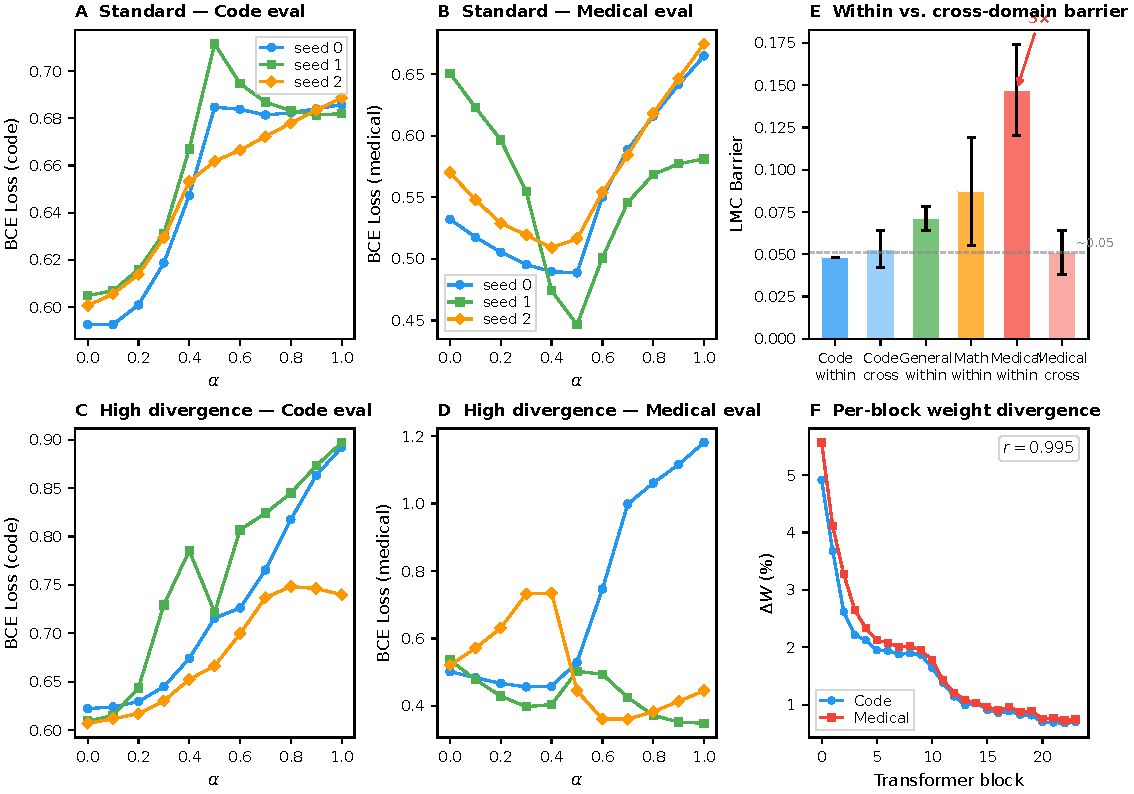
\includegraphics[width=\textwidth]{../reports/fig1_lmc_overview.pdf}
    \caption{\textbf{LMC barrier curves and comparative analysis.}
    \textbf{Panels A--D:} Loss along the linear interpolation path $\theta(\alpha) = (1-\alpha)\theta_{\text{code}} + \alpha\theta_{\text{medical}}$ for standard (A, B) and high (C, D) divergence, evaluated on code and medical test sets. Colored lines represent 3 independent seeds.
    \textbf{Panel E:} Within-domain vs.\ cross-domain barrier comparison — code models show equivalence while medical models show 3$\times$ larger within-domain barriers. Bars show mean $\pm$ 1$\sigma$.
    \textbf{Panel F:} Per-block weight divergence from pretrained checkpoint, code and medical overlaid ($r = 0.995$). Divergence concentrates in early layers and decreases roughly exponentially with depth.
    See Appendix for full numerical tables.}
    \label{fig:fig1}
\end{figure}

\begin{figure}[p]
    \centering
    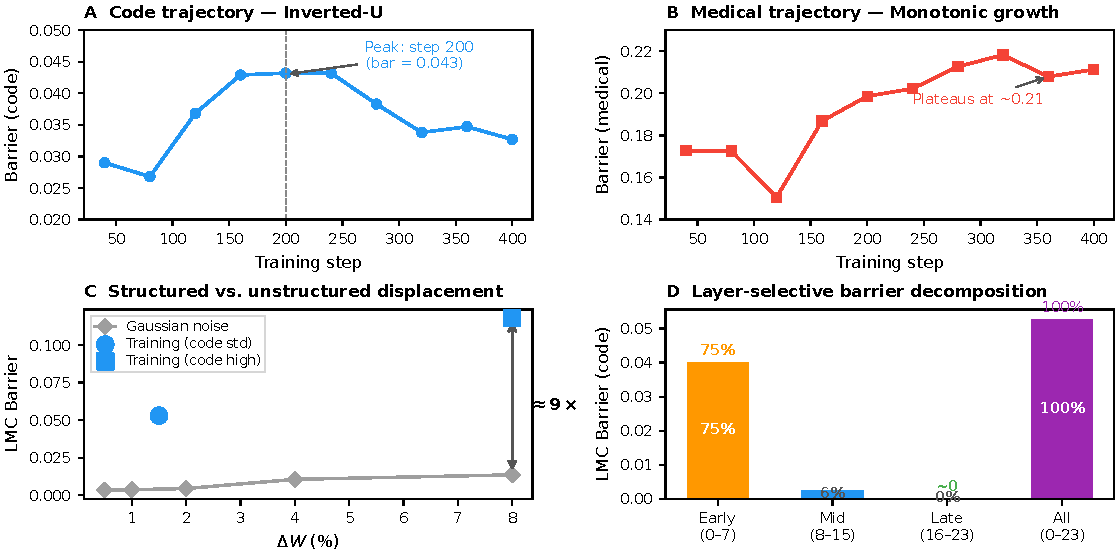
\includegraphics[width=\textwidth]{../reports/fig2_trajectory_analysis.pdf}
    \caption{\textbf{Training trajectory, Gaussian calibration, and layer-selective analysis.}
    \textbf{Panel A:} Code domain trajectory — inverted-U barrier peaking at step 200 (bar = 0.043) then declining to 0.033 at step 400, despite monotonically increasing $\Delta W$.
    \textbf{Panel B:} Medical domain trajectory — monotonic barrier growth without recovery, plateauing at $\sim$0.21 from step 320 onward.
    \textbf{Panel C:} Gaussian noise perturbation produces negligible barriers (gray) regardless of $\Delta W$ magnitude, while training-induced displacement creates barriers $\sim$9$\times$ larger at equivalent magnitude.
    \textbf{Panel D:} Layer-selective interpolation — 75\% of the barrier is concentrated in early layers (0--7), with late layers (16--23) showing near-zero penalty.}
    \label{fig:fig2}
\end{figure}

\begin{figure}[p]
    \centering
    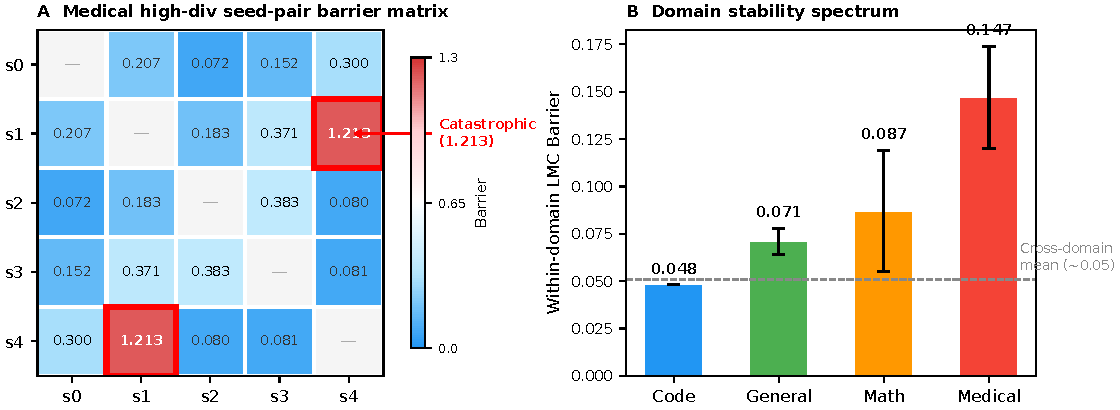
\includegraphics[width=\textwidth]{../reports/fig3_seedpair_stability.pdf}
    \caption{\textbf{Seed-pair compatibility and domain stability spectrum.}
    \textbf{Panel A:} Barrier matrix for all $\binom{5}{2} = 10$ medical high-divergence seed pairs. Cell color encodes barrier magnitude on a blue--white--red scale from 0 to 1.3. Seed s4 produces barriers from 0.080 (with s2) to 1.213 (with s1) — a 15$\times$ range depending solely on which partner it is paired with. Red boxes highlight the catastrophic s1$\leftrightarrow$s4 pair.
    \textbf{Panel B:} Within-domain LMC barriers across four domains, ordered by stability. The cross-domain mean ($\sim$0.05, dashed line) is shown as a reference, highlighting that domain difference contributes negligibly to barrier height compared to domain-specific training stability.}
    \label{fig:fig3}
\end{figure}

% ============================================================
% REFERENCES
% ============================================================
\begin{thebibliography}{99}

\bibitem{draxler2018barriers}
F.\ Draxler, K.\ Veschgini, M.\ Salmhofer, and F.\ Hamprecht.
\textit{Essentially No Barriers in Neural Network Energy Landscapes.}
In \emph{ICML}, 2018.

\bibitem{garipov2018loss}
T.\ Garipov, P.\ Izmailov, D.\ Podoprikhin, D.\ Vetrov, and A.\ G.\ Wilson.
\textit{Loss Surfaces, Mode Connectivity, and Fast Ensembling of DNNs.}
In \emph{NeurIPS}, 2018.

\bibitem{li2018visualizing}
H.\ Li, Z.\ Xu, G.\ Taylor, C.\ Studer, and T.\ Goldstein.
\textit{Visualizing the Loss Landscape of Neural Nets.}
In \emph{NeurIPS}, 2018.

\bibitem{frankle2020lmc}
J.\ Frankle, G.\ K.\ Dziugaite, D.\ M.\ Roy, and M.\ Carbin.
\textit{Linear Mode Connectivity and the Lottery Ticket Hypothesis.}
In \emph{ICML}, 2020.

\bibitem{entezari2022permutation}
R.\ Entezari, H.\ Sedghi, O.\ Saukh, and B.\ Neyshabur.
\textit{The Role of Permutation Invariance in Linear Mode Connectivity of Neural Networks.}
In \emph{ICLR}, 2022.

\bibitem{ainsworth2023git}
S.\ Ainsworth, J.\ Hayase, and S.\ Srinivasa.
\textit{Git Re-Basin: Merging Models modulo Permutation Symmetries.}
In \emph{ICLR}, 2023.

\bibitem{mirzadeh2021lmc}
S.\ I.\ Mirzadeh, M.\ Farajtabar, D.\ Gorur, R.\ Pascanu, and H.\ Ghasemzadeh.
\textit{Linear Mode Connectivity in Multitask and Continual Learning.}
In \emph{ICLR}, 2021.

\bibitem{lubana2023mechanistic}
E.\ S.\ Lubana, E.\ J.\ Bigelow, R.\ P.\ Dick, D.\ Krueger, and H.\ Tanaka.
\textit{Mechanistic Mode Connectivity.}
In \emph{ICML}, 2023.

\bibitem{izmailov2018averaging}
P.\ Izmailov, D.\ Podoprikhin, T.\ Garipov, D.\ Vetrov, and A.\ G.\ Wilson.
\textit{Averaging Weights Leads to Wider Optima and Better Generalization.}
In \emph{UAI}, 2018.

\bibitem{wortsman2022soups}
M.\ Wortsman, G.\ Ilharco, S.\ Y.\ Gadre, R.\ Roelofs, R.\ Gontijo-Lopes, A.\ S.\ Morcos, H.\ Namkoong, A.\ Farhadi, Y.\ Carmon, S.\ Kornblith, and L.\ Schmidt.
\textit{Model Soups: averaging weights of multiple fine-tuned models improves accuracy without increasing inference time.}
In \emph{ICML}, 2022.

\bibitem{wortsman2022wise}
M.\ Wortsman, G.\ Ilharco, J.\ W.\ Kim, M.\ Li, S.\ Kornblith, R.\ Roelofs, R.\ G.\ Lopes, H.\ Hajishirzi, A.\ Farhadi, H.\ Namkoong, and L.\ Schmidt.
\textit{Robust fine-tuning of zero-shot models.}
In \emph{CVPR}, 2022.

\bibitem{yadav2023ties}
P.\ Yadav, D.\ Tam, L.\ Choshen, C.\ Raffel, and M.\ Bansal.
\textit{TIES-Merging: Resolving Interference When Merging Models.}
In \emph{NeurIPS}, 2023.

\bibitem{ilharco2023editing}
G.\ Ilharco, M.\ T.\ Ribeiro, M.\ Wortsman, S.\ Gururangan, L.\ Schmidt, H.\ Hajishirzi, and A.\ Farhadi.
\textit{Editing Models with Task Arithmetic.}
In \emph{NeurIPS}, 2023.

\bibitem{matena2022merging}
M.\ Matena and C.\ Raffel.
\textit{Merging Models with Fisher-Weighted Averaging.}
In \emph{NeurIPS}, 2022.

\bibitem{jin2023dataless}
X.\ Jin, X.\ Ren, D.\ Preotiuc-Pietro, and P.\ Cheng.
\textit{Dataless Knowledge Fusion by Merging Weights of Language Models.}
In \emph{ICLR}, 2023.

\bibitem{stoica2024zipit}
G.\ Stoica, D.\ Bolya, J.\ Bjorner, P.\ Ramesh, T.\ Hearn, and J.\ Hoffman.
\textit{ZipIt! Merging Models from Different Tasks without Training.}
In \emph{ICLR}, 2024.

\bibitem{singh2020fusion}
S.\ P.\ Singh and M.\ Jaggi.
\textit{Model Fusion via Optimal Transport.}
In \emph{NeurIPS}, 2020.

\bibitem{biderman2023pythia}
S.\ Biderman, H.\ Schoelkopf, Q.\ Anthony, H.\ Bradley, K.\ O'Brien, E.\ Hallahan, M.\ A.\ Khan, S.\ Purohit, U.\ S.\ Prashanth, E.\ Raff, A.\ Skripnik, P.\ Liskovich, Q.\ G.\ Liao, N.\ Piel, A.\ Patel, A.\ Jones, L.\ Gao, and S.\ Goldfarb.
\textit{Pythia: A Suite for Analyzing Large Language Models.}
In \emph{NeurIPS}, 2023.

\bibitem{gururangan2020dapt}
S.\ Gururangan, A.\ Marasovi\'{c}, S.\ Swayamdipta, K.\ Lo, I.\ Beltagy, D.\ Downey, and N.\ A.\ Smith.
\textit{Don't Stop Pretraining: Adapt Language Models to Domains and Tasks.}
In \emph{ACL}, 2020.

\bibitem{neyshabur2020transfer}
B.\ Neyshabur, H.\ Sedghi, and C.\ Zhang.
\textit{What is being transferred in transfer learning?}
In \emph{NeurIPS}, 2020.

\bibitem{kirkpatrick2017ewc}
J.\ Kirkpatrick, R.\ Pascanu, N.\ Rabinowitz, J.\ Veness, G.\ Desjardins, A.\ A.\ Rusu, K.\ Milan, J.\ Quan, T.\ Ramalho, A.\ Grabska-Barwinska, D.\ Hassabis, C.\ Clopath, D.\ Kumaran, and R.\ Hadsell.
\textit{Overcoming catastrophic forgetting in neural networks.}
In \emph{PNAS}, 2017.

\bibitem{aljundi2018mas}
R.\ Aljundi, F.\ Babiloni, M.\ Elhoseiny, M.\ Rohrbach, and T.\ Tuytelaars.
\textit{Memory Aware Synapses: Learning what (not) to forget.}
In \emph{ECCV}, 2018.

\bibitem{fort2019stiffness}
S.\ Fort, P.\ K.\ Nowak, S.\ Jastrzebski, and S.\ Narayanan.
\textit{Stiffness: A New Perspective on Generalization in Neural Networks.}
In \emph{NeurIPS}, 2019.

\bibitem{zhang2017understanding}
C.\ Zhang, S.\ Bengio, M.\ Hardt, B.\ Recht, and O.\ Vinyals.
\textit{Understanding Deep Learning Requires Rethinking Generalization.}
In \emph{ICLR}, 2017.

\end{thebibliography}

\end{document}
